\documentclass{beamer}
\setbeamertemplate{caption}[numbered]
\usepackage{multirow}
\usepackage{fancyhdr}
\usepackage{graphicx}
\usepackage{multimedia}

\usetheme{Berlin}  %{Berlin}{Hannover}{Singapore}{CambridgeUS}

\title{Generative Adversarial Networks for Automatic Image Colorization}
\subtitle{\textbf{Team}: Yet Another Layer - YAL}


\author{Cameron Fabbri, Md Jahidul Islam}

\begin{footnotesize}

\end{footnotesize}


\begin{document}
\date{}
%%%%%%%%%%%%%%%%%%%%%%%%%%%%%%%%%
\begin{frame}
\thispagestyle{empty}
\titlepage
\end{frame}
%%%%%%%%%%%%%%%%%%%%%%%%%%%%%%%%%

\section*{Introduction}
%%%%%%%%%%%%%%%%%
\begin{frame}
\frametitle{\textbf{Image Colorization}}

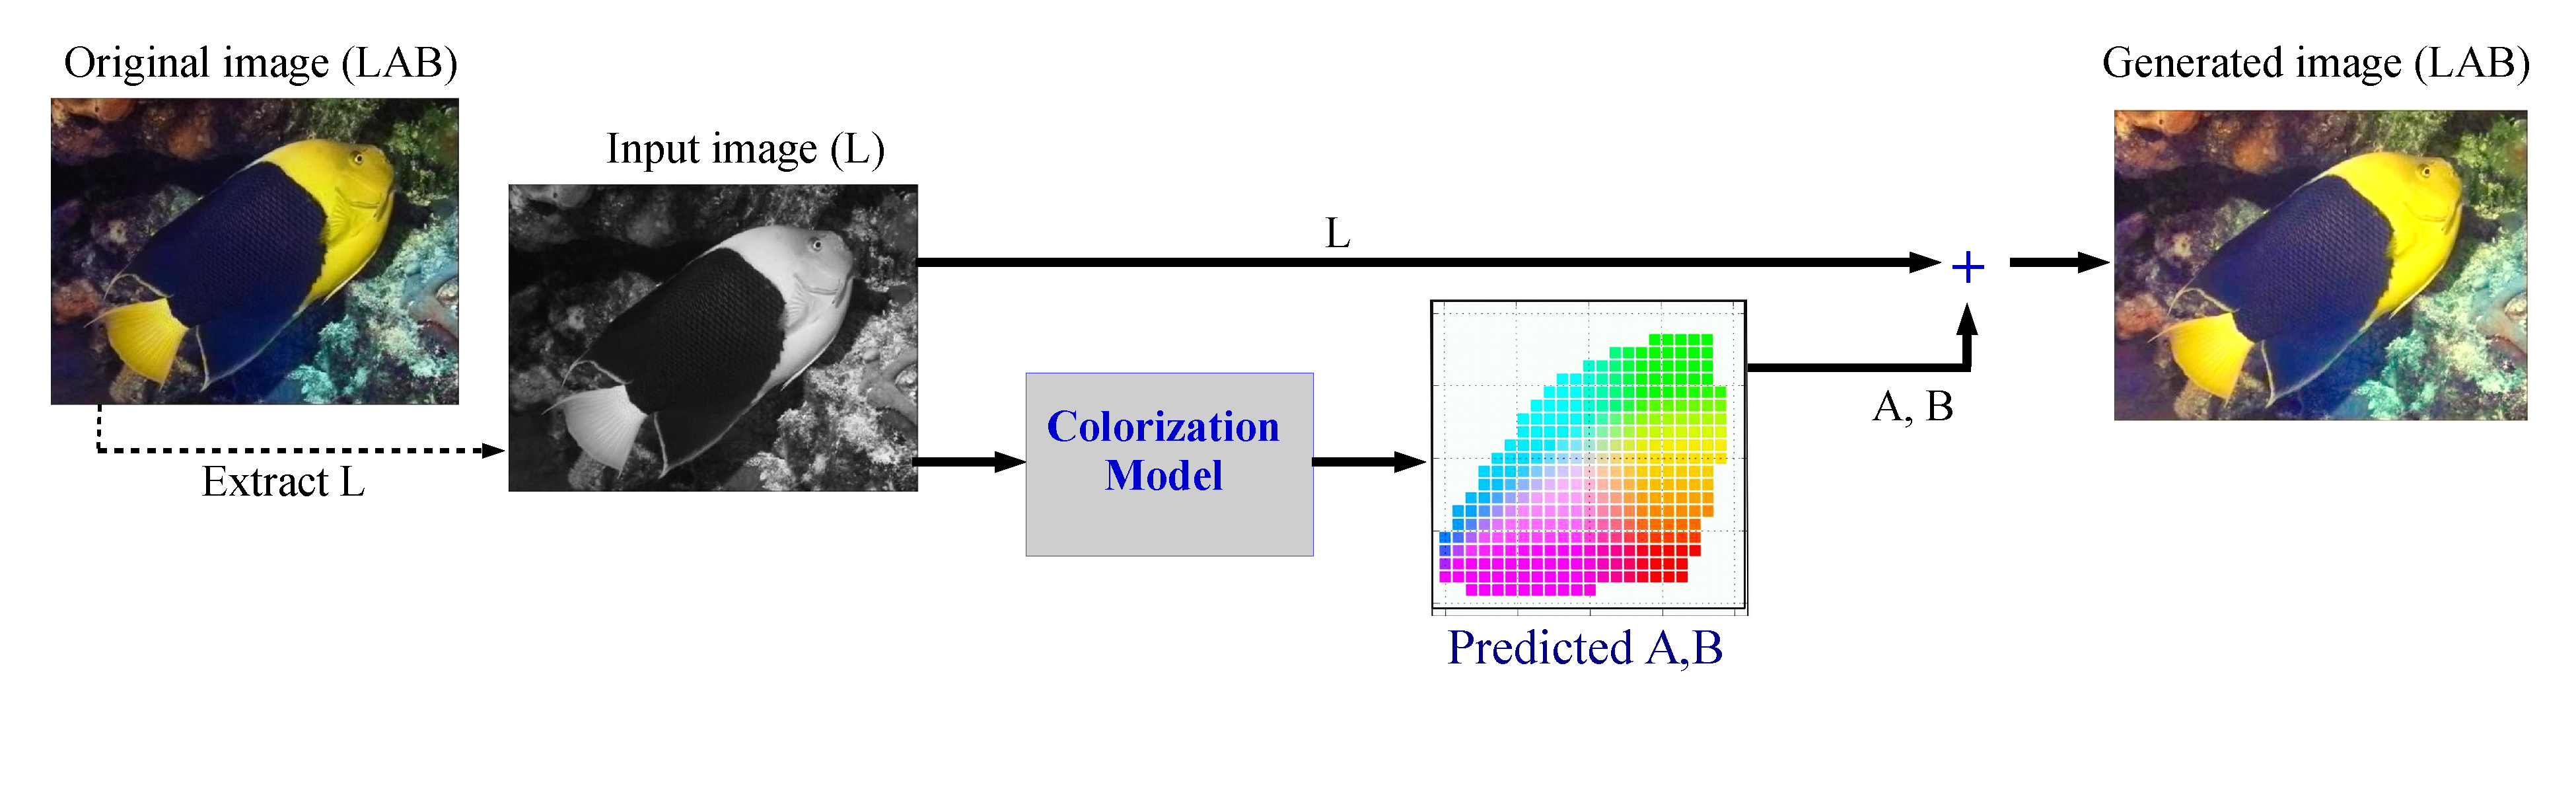
\includegraphics[width=\linewidth]{6.pdf}



\end{frame}
%%%%%%%%%%%%%%%%%%

\begin{frame}
\frametitle{\textbf{Background}}
\framesubtitle{\textbf{Applications and Approaches}}
\begin{itemize}
  \item Problem domain choices:
  
	\begin{enumerate}[$-$]
	\item  \textbf{Image-to-image translation}, Classification
	\end{enumerate}
	
	\item Color-space choices:
  
	\begin{enumerate}[$-$]
	\item  \textbf{LAB}, RGB
	\end{enumerate}
	
	
\end{itemize}

\begin{itemize}
  \item Applications
  
	\begin{enumerate}[$-$]
	\item  bla
	 \item bla
	\end{enumerate}
	
	\item Approaches
  
	\begin{enumerate}[$-$]
	\item Classical
	\item Deep learning based
	\begin{enumerate}[$-$]
	  \item Generative models
	  \item \textbf{Adversarial model}
	\end{enumerate}	 
	\end{enumerate}
	
\end{itemize}
\end{frame}
%%%%%%%%%%%%%%%%%%%%%%%


\section*{Background}

\section*{Classical and Generative Models}

\section*{GAN-based Models}

\section*{Results}



\begin{frame}
\begin{quote}
\begin{center}
\huge{Thank you all !} \\

\end{center}   
\end{quote}
\end{frame}
\end{document}